\definecolor{dkgreen}{rgb}{0,0.6,0}
\definecolor{gray}{rgb}{0.5,0.5,0.5}
\definecolor{mauve}{rgb}{0.58,0,0.82}

\lstset{frame=tb,
  language=Java,
  aboveskip=3mm,
  belowskip=3mm,
  showstringspaces=false,
  columns=flexible,
  basicstyle={\small\ttfamily},
  numbers=none,
  numberstyle=\tiny\color{gray},
  keywordstyle=\color{blue},
  commentstyle=\color{dkgreen},
  stringstyle=\color{mauve},
  breaklines=true,
  breakatwhitespace=true,
  tabsize=3
}





\chapter{Introduction}



\section{Motivation}
\label{sec:motivation}

In this day in age, technology is continuing to rapidly grow and expand. It is expected in 2020 that there will be two-hundred billion devices connected \cite{Milkovich:2013}.
With that being said, the risk of attacks is becoming even more prominent and important. SQL injection attacks make up two-thirds of all web application attacks. Major industries and companies are victims of this. In 2011 Sony was hacked by LulzSec using SQL injection. In 2013 one hundred and fifty-three million user records were stolen from Adobe and it cost them over one million in legal fees. To fully address this issue and dive into why some companies and industries are more vulnerable than others, we need to figure out what exactly a vulnerability is and how to assess it. In computer science terms, a vulnerability is simply just a weakness in a computer system or network that can be exploited. This is important because when you have a vulnerable system, your data can be breached and stolen. The next step is assessing this information. With all of this information, I am physically trying to understand why some vulnerabilities may lie within some networks more than others and I plan on doing that by using the SQL injection technique. I chose to do this because the risk of being hacked in society today is very imminent. Every thirty-nine seconds there is an attack happening \cite{Milkovich:2013}.
The odds of the majority of the people on this planet that have been hacked are very high. I want to figure out why it may be so easy for someone to hack someone else. With the collection of data, and experience that I gain, I should have a better understanding of why that may be and start creating a prototype that may help to guard against future hacks. Today, there are many tools out there that you can use to automatically assess your network or computer and give you a diagnostic of the possible vulnerabilities that your system has, and can give you suggestions on what you can do to help guard against those vulnerabilities.

I chose to do SQL injection, rather than any of the other tools or attacks because SQL injection is by far the most prominent of the vulnerabilities that are common with web applications. With a SQL injection attack, you can insert, delete and add data to a very harmful web application. Other forms of attacks can't quite be able to physically alter data. Being able to detect vulnerable spots in a company's network can save that company thousands to millions of dollars based on the size of that company. A company could be hacked any day without even realizing it. These spots in their network can be near impossible to detect by the human eye. Since this is an issue, companies need to have some sort of security measure at all times and they need to keep those measures updated. The majority of the companies that are targeted for attacks are in the healthcare, retail, and technology industries. This is the case because usually these industries either have a very relaxed security protocol or the information that they have is very important. Assessing vulnerabilities in society now is very important. There is too much valuable information nowadays online. The best way to combat your system from potential hacks is to keep yourself protected at all times and using one of these services or tools is the best way to do that. My ultimate goal was to investigate further as to why it is so easy to penetrate a system or a network and with my findings, I now understand why some systems may be more vulnerable than others and I am working on a possible solution that could help fix this hacking crisis. Please see Table ~\ref{tab:my-table} for more stats.


\begin{table}[]
\caption{Why Companies were hacked in 2021}
\centering
\begin{tabular}{|l|}
\hline
65\% of companies have over 1,000 stale user accounts                                                                                    \\ \hline
Companies protect only 3\% of their folders                                                                                              \\ \hline
75\% of all attacked businesses reported fraudulent emails                                                                               \\ \hline
\begin{tabular}[c]{@{}l@{}}32\% of black hat hackers admit privileged accounts are their\\  number one way to hack systems.\end{tabular} \\ \hline
\end{tabular}

\label{tab:my-table}
\end{table}




\section{SQL Origin Story}
\label{sec:origin story}

Let us first take a look at the origin of SQL. SQL stands for Structured Query Language and it is a programming language that is used to communicate and manipulate databases. SQL programming language was first developed in the 1970s by IBM researchers Raymond Boyce and Donald Chamberlin. The programming language then known as SEQUEL was created following the publishing of Edgar Frank Todd's paper, "A relational model of data for large shared data banks," in 1970. In his paper, Todd proposed that all data in a database be represented in the form of relations. It was based on this theory that Boyce and Chamberlin came up with SQL. In the book "Oracle Quick Guides," author Malcom Coxall writes that the original SQL version was designed to manipulate and retrieve data stored in IBM's relational database management systems known as "System R." It wasn't until several years later, however, that the SQL language was made available publicly. In 1979, a company called Relational Software, which became oracle, commercially released its version of the SQL language called Oracle V2. Since then, the American National Standards Institute and the International Standards Organization have deemed the SQL language the standard language in relational database communication. While major SQL vendors do modify the language to their desires, most base their SQL programs off of the ANSI-approved version \cite{brooks_2014}.




Rather than trying to write SQL for their databases, many companies use a database management system that has SQL already built into it. Developed and distributed by Oracle, MySQL is one of the most popular SQL database management systems currently available. The software is an open-source version, which means it can be downloaded and used for free. According to the web hosting service GoDaddy, MySQL is a sophisticated and powerful relational database used by many web applications to create and change content quickly. Currently, many of the world's largest and most well-known brands rely upon MySQL to make their web applications function properly, including Facebook, Google, Adobe, Alcatel Lucent, and Zappos. In addition to MySQL, there are several other open-source SQL database management systems, including PostgreSQL, Ingres, and Firebird. SQL is a declarative language, therefore, its syntax reads like a natural language. A SQL statement begins with a verb that describes the action, for example, SELECT, INSERT, UPDATE or DELETE. Now let us take a look at some example SQL syntax to simply show how all of this works. See the following SQL statement :

\section{SQL Examples}
\label{sec:sql examples}


\bigskip
\bigskip
\begin{lstlisting}
SELECT 
    first_name
FROM
    Employees;
WHERE
    YEAR(hire_date) = 2000;
\end{lstlisting}
\bigskip
\bigskip

As you see, it reads like a normal sentence. Get the first names of employees who were hired in 2000.
The "SELECT" "firstname", "FROM employees", and "WHERE" are clauses in the SQL statement. Some clauses are mandatory e.g., the "SELECT" and "FROM" clause whereas others are optional such as the "WHERE" clause.
Because SQL was designed specifically for the non-technical people in mind, it is very simple and easy to understand. To write a SQL statement, you just need to say what you want instead of how you want it like other imperative languages such as PHP, Java, and C++. SQL is a user-friendly language because it is mainly for the users who perform ad-hoc queries and generate reports. Nowadays, SQL is used by highly-technical people like data analysts, data scientists, developers, and database administrators.
SQL is made up of many commands. Each SQL command is typically terminated with a semicolon(;). For example, the following are two different SQL commands separated by a semicolon(;).

\bigskip
\bigskip
\begin{lstlisting}
SELECT 
    first_name, last_name
FROM
    Employees;
DELETE FROM Employees;
WHERE
   hire_date < '1990-01-01'
\end{lstlisting}
\bigskip
\bigskip

SQL uses the semicolon(;) to mark the end of a command. Each command is composed of tokens that can be literals, keywords, identifiers, or expressions. Tokens are separated by space, tabs, or newlines.

In terms of other important information, you may need to understand what SQL syntax is commenting. Commenting is pretty important when it comes to bypassing a login to access a database. Let us look at a simple example of how commenting works in SQL.

\bigskip
\bigskip
\begin{lstlisting}
SELECT 
    first_name, last_name
FROM
    Employees;
DELETE FROM Employees;
WHERE
    salary < 3000; --employees with low salary
\end{lstlisting}
\bigskip
\bigskip


To document SQL statements, you use the SQL comments. When parsing SQL statements with comments, the database engine ignores the characters in the comments. A comment is denoted by two consecutive hyphens ( --) that allow you to comment on the remaining line. To document the code that can span multiple lines, you use the multiline C-style notation ( /**/) as shown in the following statement:


\bigskip
\bigskip
\begin{lstlisting}
/* increase 5% for employees whose salary is less than 3,000 */
UPDATE employees
SET
    salary = salary * 1.05
WHERE
    salary < 3000;
\end{lstlisting}
\cite{sqltutorial}
\bigskip
\bigskip


\section{Security in Databases}
\label{sec:security in databases}

With the current way our society and the digital age is, everything is stored online in a database. Since this is the reality, we must understand that there are threats to the security associated with databases. This is super important because this can compromise anywhere from one person to billions of people all across the world. What is important to database security is the minimization of threats. Now, we can simply define a threat as a possible source of harm or danger. Let us take that definition and apply it to databases. This is saying that there is the possibility of harming the database. What does this mean exactly? We can look at what threats are concerning databases to get a better understanding. There are two types of threats that can hurt a database. There are physical and logical threats to a database. Physical threats are things like disclosure of passwords, theft, and destruction of physical storage devices for a power failure. Logical threats are things such as unauthorized access to information. This can result in gaining access to confidential information, illegal modification of data, or evening destruction of database resources. This is the type of threat we are looking into with this project. To eliminate a threat we have to put in place a security policy. There are a few different types of policies that we can choose from. First, there is an Access control policy that ensures that all direct access to the system objects proceeds according to the privileges and the access rules. Next, there is an inference policy that specifies how to protect classified information from disclosure when the information is released indirectly in the form of statistical data. Next, there is a User identification/authentication policy and this indicates the requirement for the correct number of users. Next, we have accountability and this provides the requirement for record-keeping all accesses to the database. Lastly, we have a consistent policy and this defines the states in which the database is considered valid or correct and includes the integrity of the database \cite{baraani1996security}.


\section{SQL injection Origin}
\label{sec: sql injection origin}

SQL injection techniques have been described as some of the most serious threats for Web applications. SQL injection first occurred in 1998 with the first documented vulnerability being “rain.forest.puppy” in an issue of Phrack magazine which described a Microsoft SQL server yielding possibly sensitive data through the use of commands in normal user inputs like “name” or “phone number”.
Even though it was first documented in 1998, SQL injection did not appear to garner much attention in the information security community until 2002 \cite{ryder2010sql}. 
The reason for the sudden interest in a four-year-old vulnerability may have been due to the timing of national events and the appearance of devastating viruses and worms. For example, the US had recently been attacked by terrorists using hijacked planes on September 11, 2001. Shortly thereafter, the nation’s academics, military personnel, and politicians focused on increasing physical security and cybersecurity. The new attention to cybersecurity may have prompted a critical examination of vulnerabilities that could weaken the US government or infrastructure, and SQL injection may have been highlighted as a particularly risky weakness to web applications connected to database systems. The increased attention on SQL injection in 2002 appears to reflect the rising interest in cybersecurity at the time. Noting that the viruses and worms discussed above targeted Windows systems, Bill Gates released a memo earlier that year describing the new direction of Microsoft toward Trustworthy Computing, an initiative to improve the security of computer technology and software produced by the company \cite{sun2007classification}.
In order to understand the history of a SQL injection attack, it may help to learn how the attack works. In general, the whole principle of an SQL injection attack is to simply take advantage of a poorly-coded web application to transmit commands directly to a database to gain access to that database, and then perform the operation like copying, modifying, or deleting data. Please see Figure ~\ref{fig:sql injection diagram} for a simple diagram showing this.


\section{SQL injection techniques}
\label{sec:sql injection techniques}

\begin{figure}
\centering
\smartdiagram[circular diagram:clockwise]{Hacker identifies vulnerability, sql code is input into login, Hacker has access to view delete add and alter data in database}
\caption{SQL injection diagram}
\label{fig:sql injection diagram}
\end{figure}

The way I had assessed vulnerabilities was by using a technique called SQL injection. SQL injection is simply an injection technique used to attack data-driven applications such as web applications for example while SQL is just a domain-based language for managing data in a database. A SQL injection attack occurs when an attacker changes the intended effect of a SQL query by inserting new SQL keywords or operators into the query. Within SQL injection, there are different types of injection techniques that you could possibly use. The various types are injection through user input, injection through cookies, injection through server variables, and second-order injection. To briefly explain all of these different techniques and the styles that all of these use, injection through user input is when attackers can simply inject SQL commands by providing suitably crafted user input.
Injection through cookies is when a client returns to a web application, cookies can then be used to restore the client's information \cite{W3schools}.
This is unsafe because malicious content could tamper with the cookie's contents. Injection through server variables is if there are variables that are logged to a database without sanitization, that could create a SQL injection vulnerability. Lastly, second-order injection is when attackers seed malicious inputs into a system or database to indirectly trigger a SQL injection attack when that input is used at a different time \cite{halfond2006classification}.
These types of techniques relate to vulnerabilities because you can use an injection attack on a web application and assess the vulnerabilities related to the web application first-hand. I chose to do SQL injection because it will allow me to learn new skills while also experiencing a deeper level of security and the measures that are taken to ensure security. There are a few other techniques that you can use to assess vulnerabilities within the computer science field. Some of those techniques include baseline reporting, code review, and attack surface review. In essence, all of these techniques rely on you to physically go into your system or network and sift through the code to see if you can find any bugs or errors. As it stands now, being able to assess vulnerabilities is important if you want to ensure that your information is safe. Let us walk through a sample injection attack to see what exactly this could look like.


\section{SQL injection example}
\label{sec:sql injection example}


\bigskip
\bigskip
\begin{lstlisting}
SELECT
    *
FROM
    accounts
WHERE
    custID = "" + request.getParamater("id") + ""
\end{lstlisting}
\bigskip
\bigskip
\begin{sloppypar}
The attacker can modify the 'id' parameter value in 
the browser field to send ' or '1'='1;.This could be done by typing a web application address like :http://example.com/app/accountView?id=' or '1'='1. 
In this case, the entry changes the meaning of the query 
to return all the records from the accounts table 
which can lead to unauthorized disclosure of confidential 
or private information \cite{horner2017sql}.
\end{sloppypar}
\section{Assessment Services}
\label{sec: assessment services}


There are types of assessment services out there as well that can assess your computer for vulnerabilities. Some of those assessment services are network mapping, vulnerability scanning, and web application assessment. In tangent with possible assessment services that one may use, there are also assessment tools that one can use to help with checking their system or network with possible vulnerabilities. Some of the tools are manual testing, automated testing, fuzz testing, black box testing, grey box testing, and white box testing. To briefly go over these techniques as well, manual testing is when the tester doesn't use any software or tool but actually just uses their own knowledge and experience to find the vulnerabilities within the system \cite{SoftwareT}.
Automated testing is when you simply use an automated vulnerability testing tool to find out possible vulnerabilities in the system \cite{automate2006}.
Fuzz testing is when the user inputs invalid or random data into the system to see if there are any crashes or failures \cite{fuzzmisc}.
Black box testing is when the tester performs on networks but in this technique, the tester does not have any prior knowledge of the network architecture or systems.
In grey box testing, it is the same as black-box testing except the tester has some knowledge of the testing network.
Lastly, in white box testing, it is the same as both black and grey box except that in this technique, the tester has complete knowledge of the testing network and its configurations \cite{goel2015vulnerability}.
All of these services and tools allow for the programmer to scan their data to make sure that there has not been any breaches and that their systems aren't too vulnerable.

\section{VPN Services}
\label{sec:VPN services}



Let us take a closer look at what a VPN is and what it does. As stated previously, A VPN is a virtual private network but what does that really mean? a VPN is a network; that is, it provides inter-connectivity to exchange information among various entities that belong to the VPN. Secondly, it is private, that is, it has all the characteristics of a private network \cite{venkateswaran2001virtual}.
As we can see, from this definition, a VPN can be very useful to use in terms of helping us create a prototype that revolves around keeping someone's private data private. Because of the privacy factor, VPN's have become pretty popular today in society as they are also relatively cheap. There are, however, a few different types of VPN services though. Specifically, there are three and they are Local Area Network Interconnect VPN services, Dial-up VPN services, and Extranet VPN services. Let us take a closer look at these. Let's first start with LAN Interconnect VPN services. Please see Figure ~\ref{fig:lan interconnect VPN}

\bigskip
\begin{figure}[hbt!]
\centering
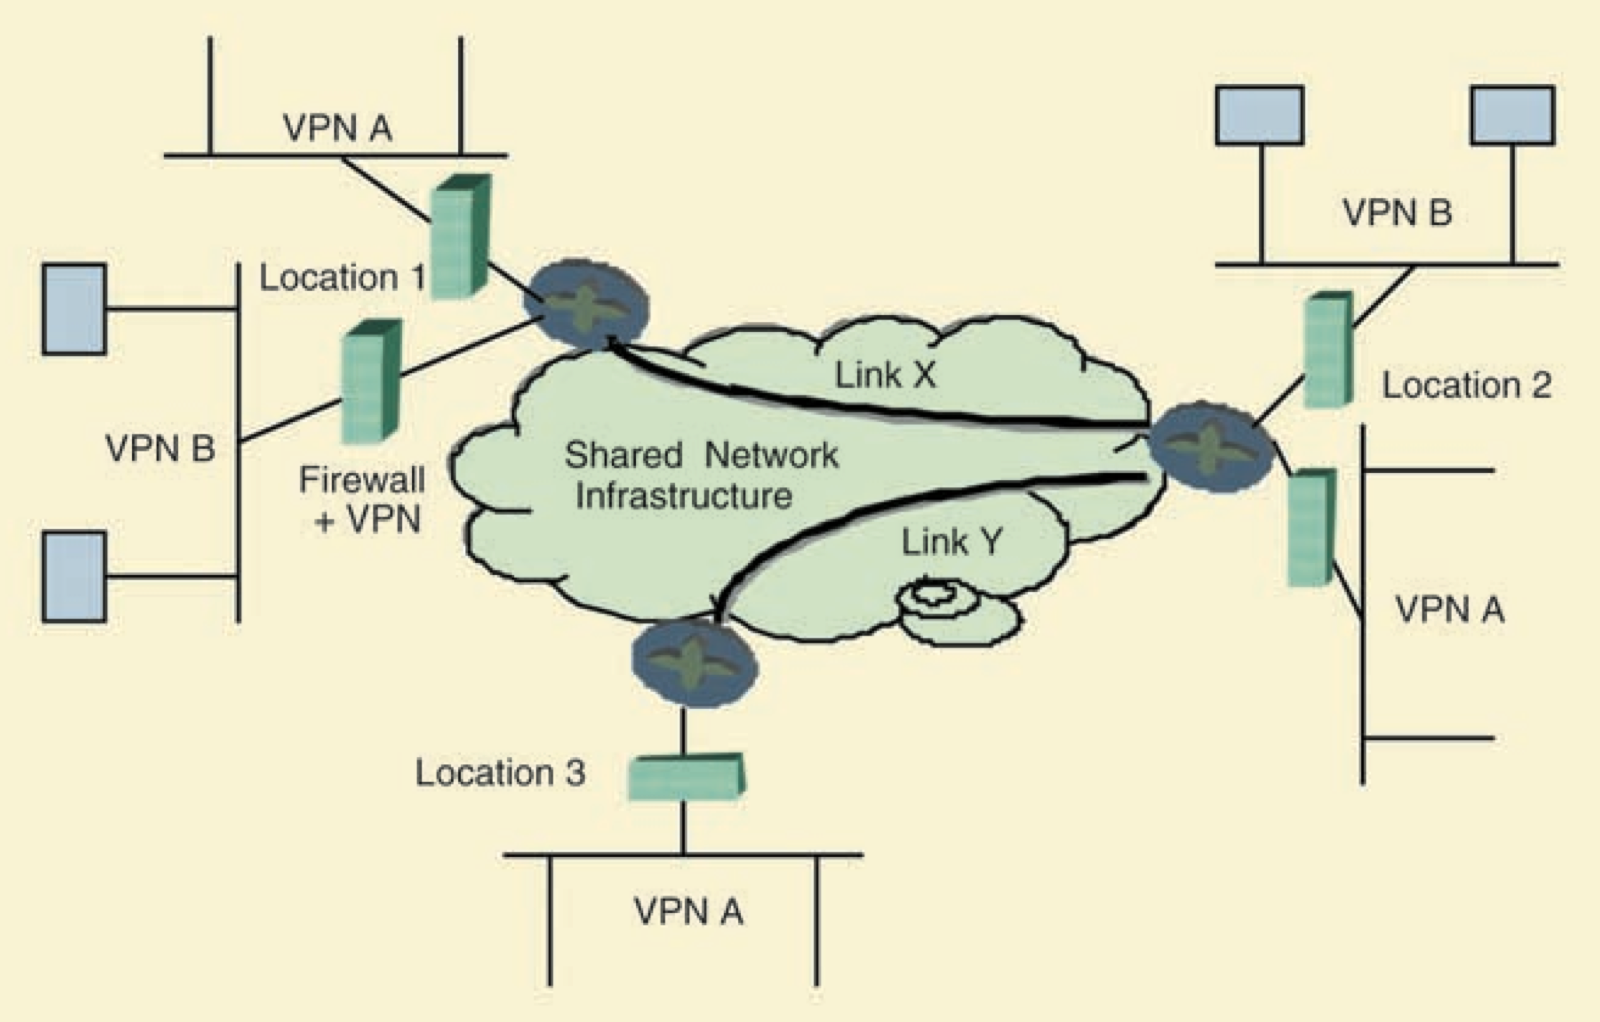
\includegraphics[width=5in]{../images/LAN-interconnect-VPN.png}%
\caption{LAN Interconnect VPN}
\label{fig:lan interconnect VPN}
\end{figure}
\bigskip

LAN Interconnect VPN services help to interconnect local area networks located at multiple geographic areas over the shared network infrastructure. Typically, this service is used to connect multiple geographic locations of a single company. Several small offices can be connected with their regional and main offices. This service provides a replacement for the expensive dedicated links. A simple LAN interconnect example is shown in the figure. VPN A has sites in geographic locations 1, 2, and 3, while VPN B has sites in geographic locations 1 and 2. Both vpns A and B are implemented on top of a shared network infrastructure. The advantage is the flexibility it offers \cite{venkateswaran2001virtual}.
Next, let us take a look at Dial-up VPN services. Please see Figure ~\ref{fig:Dial-up VPN}

\bigskip
\begin{figure}[hbt!]
\centering
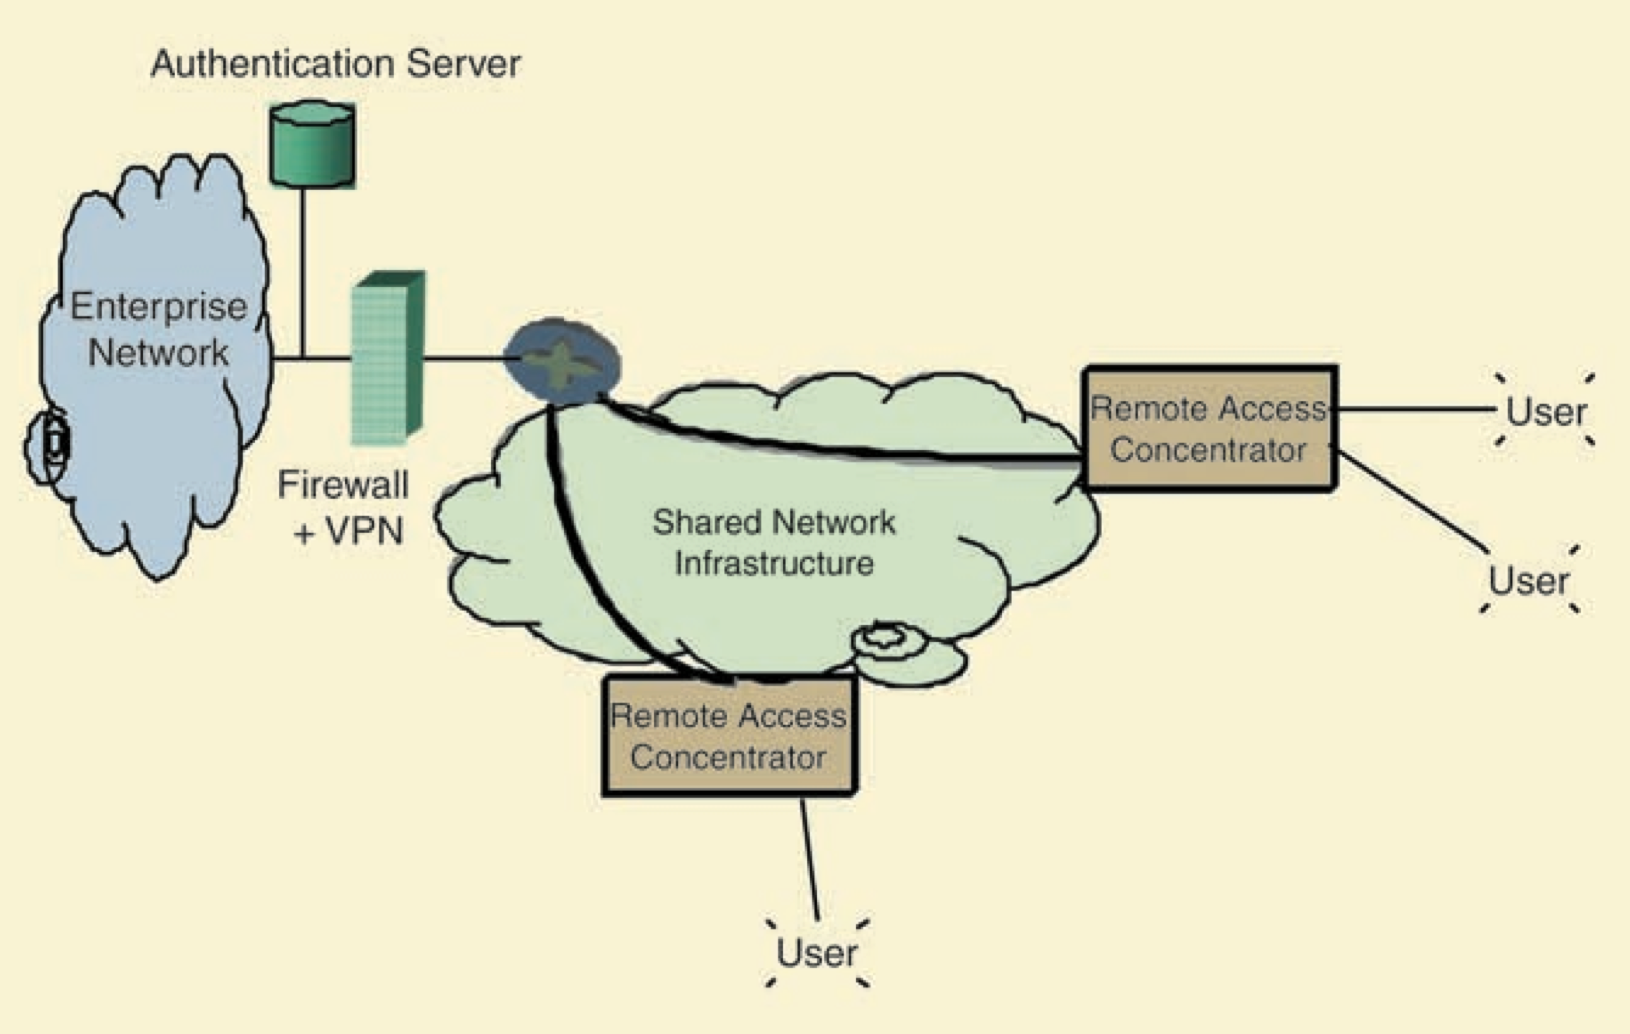
\includegraphics[width=5in]{../images/Dial-up-VPN.png}%
\caption{Dial-up VPN}
\label{fig:Dial-up VPN}
\end{figure}
\bigskip

From this diagram, we can see it is a bit different from the LAN VPN services. There is no VPN A or VPN B. Instead in this diagram the user is dialing into the closest remote access concentrator, which then connects to the shared network infrastructure and tries to make a clear connection to the VPN before it can have access to the server. Lastly, let us take a look at the Extranet VPN service. Please see Figure ~\ref{fig:Extranet VPN}

\bigskip
\begin{figure}[hbt!]
\centering
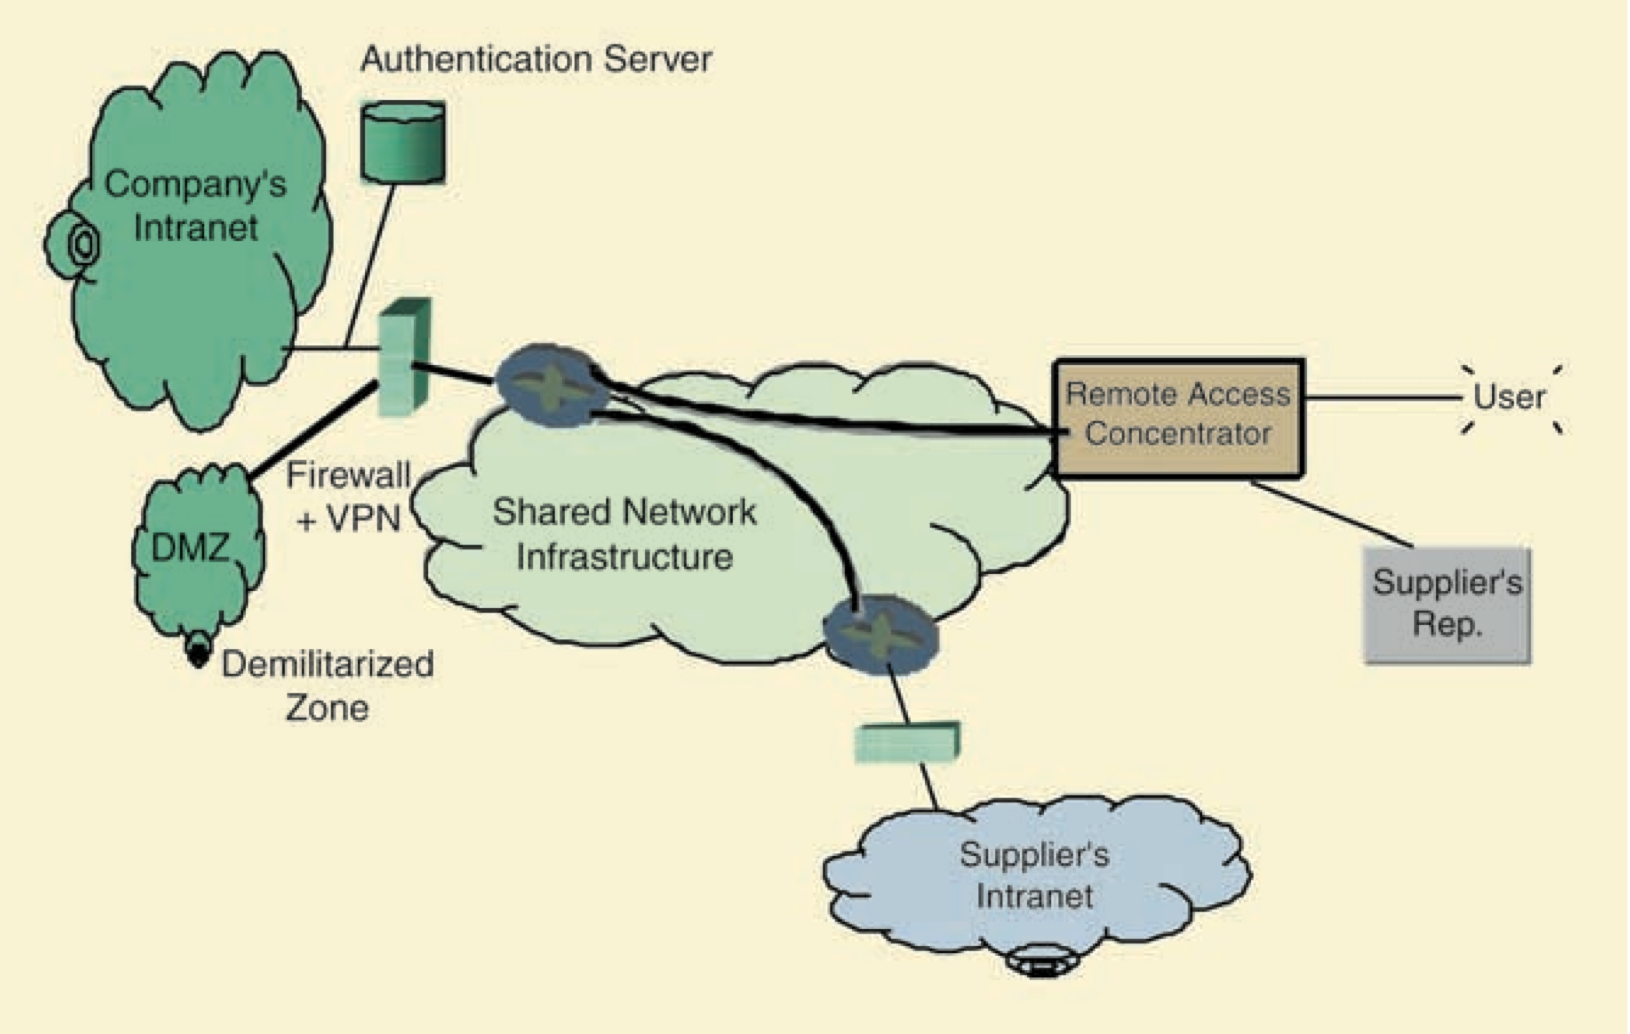
\includegraphics[width=5in]{../images/Extranet-VPN.png}%
\caption{Extranet VPN}
\label{fig:Extranet VPN}
\end{figure}
\bigskip

An Extranet VPN service shown in the figure combines the architecture of LAN Interconnect VPN services and dial-in VPN services. This infrastructure enables external vendors, suppliers, and customers to access specific areas of the company’s Intranet. The allowed specific area is denoted as the Demilitarized Zone (DMZ). When a packet is created by encapsulating and encrypting the original IP packet. The encryption keys and the algorithm parameters are negotiated and exchanged between the two VPN nodes using the Internet Key Exchange (IKE) protocols \cite{venkateswaran2001virtual}.


\section{Cloud Computing}
\label{sec:cloud computing}


Let us also try and understand more about cloud computing software. cloud computing software is something that we are all familiar with. Services such as Google, Amazon, and Microsoft all use cloud computing for their services. What exactly is it though? cloud computing is simply the availability of services in the cloud. The cloud computing idea emerges as a new computing paradigm that aims to provide reliable, customized, and QoS (quality of service) guaranteed dynamic computing environments for end-users \cite{wang2010cloud}.
Now that we know what cloud computing is, well what does it do? It allows infrastructures from the cloud to run their applications inside. There are three fundamental aspects of cloud computing. There is Hardware as a Service (Haas), Software as a service (Saas), and Data as a Service (Daas). Haas is when users buy IT hardware or in some cases even entire data centers using a subscription such as Amazon EC2. Saas is when the software or an application is hosted as a service. This eliminates the need for customers to download applications to their local computers. A modern example of this is Google Stadia's infrastructure or Spotify. Lastly, Daas is when data of any format can be accessed by users on a network. A big example of this is Google Docs \cite{wang2010cloud}.
All of these connect to the infrastructure (Iaas) which is then connected to the application. Please see Figure ~\ref{fig:Cloud Computing}


\bigskip
\begin{figure}[hbt!]
\centering
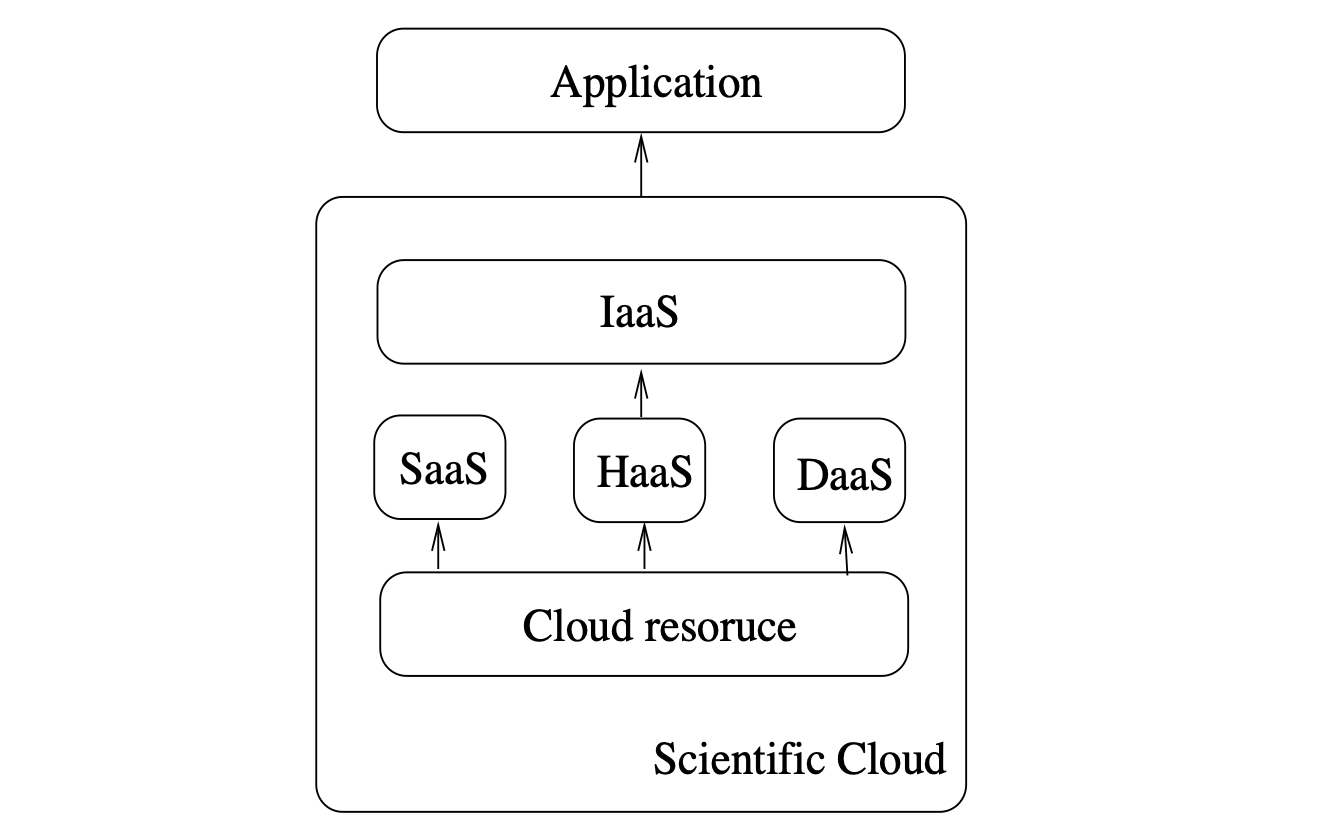
\includegraphics[width=5in]{../images/Cloud-Computing.png}%}
\caption{Cloud Computing}
\label{fig:Cloud Computing}
\end{figure}
\bigskip



\section{Goals of the Project}
\label{sec:goals}

The goal of this project is to show that vulnerabilities are a real problem in society today and this is something that we have to work towards fixing. Not only is the goal to show that these problems exist, but also to show that exploiting these problems is not as challenging as people make them seem to be. The result of someone being able to bypass login and infiltrate a database to extract valuable data is the result of sloppy code. When dealing with sensitive information like this, we cannot afford to let sloppy code be the downfall and have the possibility of somebody's sensitive information being stolen. There have been so many attacks that have been the result of sloppy code written in SQL and because of this, I have started to create my prototype that should help to mitigate against SQL injection attacks aimed at databases. My prototype simply just creates extra layers of protection that would make it much more difficult for someone to try and break into. With the use of VPN and cloud computing, it will add more layers of security because the VPN will hide your IP address from your ISP (Internet Service Provider) so people won't know where you will be logging in from and with the cloud computing structure, it will help keep your database from being accessed from unknown people or servers as you can create your server and manage who has access and who does not.


\section{Thesis Outline}
\label{sec:outline}

I carried out my proposed topic by performing a SQL injection attack on a web-based application with a database connected to it as this will allow me to get a clearer understanding of just the types of vulnerabilities that are prominent in web application and a database as it will show me just how dangerous a SQL injection attack can be. Performing a SQL injection attack showed me the security side of computer science which is very important since security is something that society as a whole benefits from. Since I did an attack on a web application, I had to make sure the web application that I performed the attack on didn't have any valuable data as I could have potentially ruined that data. After that, I had to start using SQL as a database and start using queries to be able to attack the web application and gain access to the data. For this proposed project, I attacked a web application using SQL injection with the hopes to concoct possible solutions to mitigate against vulnerabilities. I then started creating my prototype using cloud computing and VPN services as this will then help ensure more security as the database that is being accessed through the cloud won't be sitting on a dedicated server. The VPN will allow for more privacy for the user so their location services will not be revealed as a VPN changes your IP address and your online activity cannot be tracked. This will help protect the user so that nobody can track what they're doing or what web applications they are visiting. This then will help ensure the security of the user because if nobody can track your location or what web applications you might be visiting, then nobody will know that you are accessing a database through the cloud. With the knowledge I gained from being able to do a SQL injection attack, I will continue making my prototype that will help mitigate the risk of a hacker being able to use SQL injection to bypass a web application.
